\begin{center}
	\Large{\textbf{
Czech Technical University in Prague\\
Faculty of Nuclear Sciences and Physical Engineering\\ 
%Department of Physical Electronics\\
}}
 \vspace{3cm}

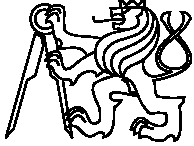
\includegraphics[width=5cm]{img/LogoCVUT}
\vspace{2cm}

\huge{\textbf{\scshape Doctoral thesis}}\\
\vspace{5mm}
{\LARGE\textbf{Metamaterials for the terahertz spectral range\\}}
\end{center}

\date{ } 			


 \vfill
\begin{minipage}{.99\textwidth}
\Large{\textbf{Prague 2016}} \hfill \Large{\textbf{Ing. Filip Dominec}}
\end{minipage}


\thispagestyle{empty} \newpage ~ \thispagestyle{empty} \newpage \setcounter{page}{1}

% --------------------------------------------------------------------------------
{\let\clearpage\relax\chapter*{Bibliografický záznam}}
 %\begin{tabular}{rl}
 %Author: 	&\textbf{Filip Dominec}\\
 %Advisor: 	&\textbf{Mgr. Filip Kadlec, Dr.}\\
 %Consultant: 	&\textbf{Doc. Ing. Ivan Richter, Dr.}\\ 
 %Year:		&\textbf{2015}\\
 %\end{tabular}

\bgroup \def\arraystretch{1.5}
\noindent\begin{tabular}{p{.30\linewidth}p{.65\linewidth}}
	Autor:				&\textbf{Ing. Filip Dominec} \\ 
					~	&České vysoké učení technické v Praze\\ 
					~	&Fakulta jaderná a fyzikálně inženýrská\\  
					~	&Katedra fyzikální elektroniky\\
Název práce:			&\textbf{Metamateriály pro terahertzovou spektrální oblast} \\
Studijní program:		&\textbf{Aplikace přírodních věd} \\
Studijní obor:			&\textbf{Fyzikální inženýrství} \\
Školitel:				&\textbf{Mgr. Filip Kadlec, Dr.} \\
					~	&Fyzikální ústav\\ 
					~	&Akademie věd České republiky\\  %Na Slovance 2,  182 21 Praha 8, Czech Republic 
Školitel specialista:	&\textbf{Doc. Ing. Ivan Richter, Dr.} \\
					~	&České vysoké učení technické v Praze\\ 
					~	&Fakulta jaderná a fyzikálně inženýrská\\  
					~	&Katedra fyzikální elektroniky\\
Akademický rok:			&\textbf{2015/16} \\			%% TODO is this the correct format?
Počet stran:			&\textbf{\pageref{enddocument}} \\  %% TODO shall give the overall page number or just that of the authored text?
Klíčová slova			&\textbf{metamateriály, fotonické krystaly, terahertzová technologie, elektrodynamické simulace, homogenisace efektivních prostředí} \\
\end{tabular}
\egroup

\thispagestyle{empty} \newpage ~ \thispagestyle{empty} \newpage \setcounter{page}{1}

% --------------------------------------------------------------------------------
{\let\clearpage\relax\chapter*{Bibliographic entry}}
\bgroup \def\arraystretch{1.5}
\noindent\begin{tabular}{p{.30\linewidth}p{.65\linewidth}}
Author:					&\textbf{Ing. Filip Dominec} \\
					~	&Czech Technical University in Prague\\
					~	&Faculty of Nuclear Sciences and Physical Engineering\\ 
					~	&Department of Physical Electronics\\
Title of Dissertation:	&\textbf{Metamaterials for the terahertz spectral range} \\
Degree Programme:		&\textbf{Applications of natural sciences} \\
Field of Study:			&\textbf{Physical engineering} \\
Supervisor:				&\textbf{Mgr. Filip Kadlec, Dr.} \\
					~	&Institute of Physics\\ 
					~	&Academy of Sciences of the Czech Republic\\  %Na Slovance 2,  182 21 Praha 8, Czech Republic 
Supervisor specialist:	&\textbf{doc. Ing. Ivan Richter, Dr.} \\
					~	&Czech Technical University in Prague\\ 
					~	&Faculty of Nuclear Sciences and Physical Engineering\\  
					~	&Department of Physical Electronics\\
Academic Year:			&\textbf{2015/2016} \\
Number of Pages:		&\textbf{\pageref{enddocument}} \\
Keywords				&\textbf{metamaterials, photonic crystals, terahertz technology, computational electrodynamics, homogenisation of effective media} \\
\end{tabular}
\egroup
\thispagestyle{empty} \newpage  ~ \thispagestyle{empty} \newpage \setcounter{page}{1}

% --------------------------------------------------------------------------------

\vspace{-20mm}
{\let\clearpage\relax\chapter*{Abstrakt}}
\noindent 
Při interakci elektromagnetických vln s periodickými strukturami lze pozorovat neobvyklé jevy, jako jsou záporný index lomu, fotonický zakázaný pás nebo silná prostorová disperze. Tyto struktury lze navrhnout tak, aby se chovaly žá\-dou\-cím způsobem, a označují se jako metamateriály nebo jako foto\-nic\-ké krys\-taly. Část z jejich navrhovaných využití je v~technice terahertzových vln, kde můžou překlenout po\-měr\-ně slabé možnosti kla\-sických součástek.  

Teoretický základ práce vychází z elektrodynamiky prostředí s frek\-ven\-ční dis\-per\-zí, která je dále zobecněna na prostředí s prostorovou disperzí a na Blochovu-Floquetovu teorii vln v~periodických strukturách. Závěr teoretické části se pokouší vyjasnit pojmy používané v~literatuře a ukázat, že myšlenky metamateriálů i foto\-nic\-kých krystalů jsou ve skutečnosti starší, než se často uvádí.

Obecná teorie je doplněna příklady terahertzového chování různorodých periodických struktur, které bylo vypočteno metodou konečných diferencí v~časové doméně (FDTD). V~některých případech byly její výsledky podloženy jinými simulačními algoritmy nebo měřeními pomocí terahertzové spektroskopie v~časové doméně.

Srovnání  různých struktur si klade za cíl srozumitelnou formou prezentovat a vy\-svět\-lit nej\-pod\-stat\-něj\-ší principy. Podobné srov\-nání zřejmě v~dosavadní literatuře chy\-bě\-lo. Klíčové vý\-sledky spočí\-vají v~popisu přechodu mezi režimy metamateriálu a fotonického krystalu v~periodickém poli dielektrických tyčinek a v~důkazech toho, že k popisu chování řady uvedených struktur je zcela nezbytné uvažovat prostorovou dispersi. V~neposlední řadě práce dokládá možnosti simulačních skriptů, které autor vyvinul a uveřejnil na internetu s úmyslem podpořit další výzkum v~této oblasti. 

\vspace{0mm}

\thispagestyle{empty} \newpage ~ \thispagestyle{empty} \newpage \setcounter{page}{1}

{\let\clearpage\relax\chapter*{Abstract}}
\noindent
Unusual phenomena such as negative index of refraction, photonic band gaps, or strong spatial dispersion are observed when electromagnetic waves interact with periodic structures. These can be designed to manipulate the wave in an advantageous way, and are known either as metamaterials or photonic crystals. Part of their proposed applications are for the terahertz technology, where they may address relatively poor performance of classical components.

The theoretical background is derived from the electrodynamics of media with classical dispersion, which is later generalized to spatially dispersive media and to the Bloch-Floquet theory of waves in periodic structures. The end of the theoretical part attempts to clarify the terminology used in the literature, and to show that the concepts of metamaterials and photonic crystals are in fact older than is sometimes assumed.

The general theory is complemented with examples of the behaviour of diverse periodic structures in the terahertz range, which was numerically simulated by the finite-difference time-domain method. In some cases, the results of this simulation method were supported by other simulation algorithms or by the experimental measurement by the terahertz time-domain spectroscopy. 

The comparison of different structures encompassed in this thesis attempts to present and explain most relevant principles in a didactic way. Arguably, such a comparison was missing in the previous literature.
The key results are in the description of the transition between metamaterial and photonic crystal regimes in a periodic array of dielectric rods, and in the demonstration of the fact that considering spatial dispersion is essential for the description of the behaviour of many periodic structures.
Last but not least, the thesis demonstrates the capabilities of the simulation environment which the author developed and completely published online to stimulate further research in this field. 

% TODO Z abstraktu musí být zřejmé, co je cílem předložené práce a jakých vědeckých výsledků doktorand osobně dosáhl.
%% + attention was focused to the parts of different topics, where the author's work could contribute with new knowledge
%\endgroup


\thispagestyle{empty} \newpage ~ \thispagestyle{empty} \newpage \setcounter{page}{1}
% --------------------------------------------------------------------------------

{\let\clearpage\relax\chapter*{Acknowledgements}}
Preparation of this thesis was not without difficulties. However, it appears that overcoming such difficulties is essential to gain some sort of valuable knowledge that cannot be conveyed through textbooks, and of experience that cannot be gained through straightforward and focused work only.  At the first place I wish to express thanks to my advisor, Dr. Filip Kadlec, and all other people who helped this project to be finished, namely Dr. Christelle Kadlec and doc. Petr Ku\v{z}el  from the Institute of Physics, and doc. Ivan Richter from the Faculty of Nuclear Engineering and Physical Sciences, Czech Technical University. 

Discussions with doc. Lukáš Jelínek and prof. Jan Macháč convinced me about the value in proper handling of the theoretical background, which later proved essential for explaining the results of the thesis. During my stay in France in 2013, the collaboration with Dr. Mathias Vanwolleghem not only greatly contributed to my experience with the numerical simulations, but presented also a great motivation for me. 

Almost surprisingly, all my scientific aspirations found a permanent and selfless support from all my family members, who always had patience with my focusing on abstract problems instead of the more practical aims and with my stubborn attitude towards some of their good advices.

The numerical results presented in the thesis could be hardly obtained without the work of hundreds of volunteers contributing to the open-source scientific software: Most of the plots were made using the Matplotlib library \cite{hunter2007} and computations were based on MEEP \cite{oskooi2010meep} and MPB programs \cite{johnson2001mpb}. 

This work was financially supported by the Czech Science Foundation under Grant No. 14-25639S.

\thispagestyle{empty} \newpage ~ \thispagestyle{empty} \newpage \setcounter{page}{7}
